% SEWS - IEEE conference paper (IEEEtran). Compile on Overleaf: upload this file and the figures/ folder.
% Placeholders in [square brackets] must be filled in by the team before submission.
\documentclass[conference]{IEEEtran}
\usepackage{cite}
\usepackage{amsmath}
\usepackage{graphicx}
\usepackage{booktabs}
\usepackage{url}

\begin{document}

\title{SEWS: A Leakage-Safe, Auditable Early-Warning System for Student Success, Evaluated on Three Public Datasets}

\author{
\IEEEauthorblockN{[Author 1]}
\IEEEauthorblockA{\textit{[Department]}\\ \textit{[College]}\\ [City], India\\ [email]}
\and
\IEEEauthorblockN{[Author 2]}
\IEEEauthorblockA{\textit{[Department]}\\ \textit{[College]}\\ [City], India\\ [email]}
\and
\IEEEauthorblockN{[Guide]}
\IEEEauthorblockA{\textit{[Department]}\\ \textit{[College]}\\ [City], India\\ [email]}
}

\maketitle

\begin{abstract}
Early-warning systems aim to identify students at risk of failing or dropping out while support can still help,
but published results are often inflated by information leakage and random test splits, and rarely report
calibration or fairness. We present SEWS, a student early-warning and intervention system that builds every
feature only from information available on the decision day, verifies this automatically, evaluates models on
later cohorts than they were trained on, explains each estimate and routes it to a mentor who decides on support.
On the Open University Learning Analytics Dataset (32,593 registrations), ten hypotheses fixed before testing were
all supported after Holm correction: ROC-AUC rose from 0.704 to 0.818 between days 30 and 90 on the same students,
six assignment features carried more unique information than all 17 platform-engagement features, and calibration
degraded on every unseen module. A weekly longitudinal study (757,357 student-weeks) found that 18 trend and
change-point features and recurrent or convolutional sequence models did not materially improve on gradient-boosted
trees (test PR-AUC 0.754--0.775 for all models), but that alert design matters: a threshold tuned per student-week
alerted 85\% of students who later passed. On a Portuguese university dataset, first-semester results raised
dropout PR-AUC from 0.555 to 0.797, and a LASSO model was statistically indistinguishable from XGBoost. At-risk
women were missed more often than men on two of the three datasets. All results use benchmark data; SEWS is at
technology readiness level 4.
\end{abstract}

\begin{IEEEkeywords}
learning analytics, early warning system, student dropout, data leakage, fairness, explainable AI
\end{IEEEkeywords}

\section{Introduction}
Indian higher education enrolled about 4.33 crore students in 2021--22 across 1,168 universities and 45,473 colleges
\cite{aishe}. At this scale a mentor cannot follow every student closely, and warning signs --- falling attendance,
missed assignments, declining marks --- are scattered across systems and noticed late. Early-warning systems
address this by estimating each student's risk from institutional records and alerting staff \cite{arnold2012,
jayaprakash2014, herodotou2019}.

Three problems limit the evidence. First, results are easily inflated by \emph{leakage} --- features that use
information not yet available at prediction time --- and by random rather than time-ordered splits
\cite{kaufman2012, le2026}. Second, few systems report whether probabilities are calibrated or whether errors fall
unequally on student groups \cite{gardner2019, baker2022}. Third, most evidence comes from UK, US and online-course
data rather than semester-based Indian colleges.

This paper makes four contributions: (1) SEWS, a working system (mobile app and website, secure database, batch
jobs, model training from an institution's own past terms with human approval) built around as-of features and an
automatic leakage guard; (2) a pre-registered evaluation of ten hypotheses on the Open University Learning Analytics
Dataset (OULAD) \cite{kuzilek2017}; (3) a weekly longitudinal study comparing tabular, sequence and survival models
and alert policies; and (4) replications on two Portuguese datasets \cite{realinho2021, cortez2008}.

\section{Related Work}
Purdue's Course Signals combined grades and learning-platform activity into traffic-light alerts \cite{arnold2012};
the Open Academic Analytics Initiative built an open-source early-alert model and studied its use across
institutions \cite{jayaprakash2014}; the Open University's predictive analytics supported teachers in large online
courses \cite{hlosta2017, herodotou2019}. Reviews identify learning-platform activity and assessment results as the
most consistent predictors \cite{namoun2021, gardner2018}, and show that prediction quality varies across time and
groups \cite{glandorf2024}. Leakage \cite{kaufman2012} and ignoring when information becomes available \cite{le2026}
inflate reported accuracy. Tree ensembles such as XGBoost \cite{chen2016} are strong predictors but often poorly
calibrated \cite{niculescu2005}. Fairness audits by subgroup slicing \cite{gardner2019}, the debate on whether
protected attributes belong in models \cite{yu2021}, and reviews of algorithmic bias \cite{baker2022} and of
explainable AI in education \cite{khosravi2022} motivate our design. SHAP \cite{lundberg2017} provides
per-prediction explanations.

\section{System}
SEWS is one Flutter codebase that runs as a mobile app and a website, backed by a PostgreSQL database (Supabase)
in which every table is protected by row-level security: a student can read only their own record and a mentor
only their caseload. Clients hold only a publishable key; secret keys are rejected at build and start-up. Batch
jobs score students, generate rule-based intervention suggestions, measure intervention outcomes, monitor drift and
deliver notifications. A training service learns from an institution's own completed terms by replaying its
history in event time; resulting models are registered as \emph{development} and reach students only after a
person approves them, with calibration evidence and a subgroup audit. Models trained on benchmark or synthetic data
can never be approved for real students. Every suggestion is reviewed by a mentor before a student sees it.

\section{Methodology}

\subsection{Data}
OULAD \cite{kuzilek2017} records 32,593 registrations of 28,785 students on 7 modules over four presentations
(2013B, 2013J, 2014B, 2014J), with learning-platform clicks, assessment submissions and scores, and the final result.
The academic outcome is Fail or Withdrawn. We train on 2013B and 2013J, tune on 2014B and test once on 2014J.
UCI~697 \cite{realinho2021} describes 4,424 students of a Portuguese polytechnic with enrolment data, first-year
semester results and the outcome (dropout 32.1\%); UCI~320 \cite{cortez2008} describes 649 (Portuguese course) and
395 (Mathematics) secondary-school students with period grades. Neither records a calendar year, so UCI~697 uses a
stratified hold-out (3,096 / 664 / 664 students) and UCI~320 $5\times5$ repeated cross-validation; these results
are not out-of-time. Demographic attributes are never model inputs; they
are used only to audit errors. Variables whose recording time was undocumented (fee status; yearly absences) were
excluded from the main models.

\subsection{As-of features and leakage guard}
Every feature is computed \emph{as of} a decision point (days 30, 60, 90; or the end of week $k$), using only
records dated on or before it; assessment scores are used only after an assumed release lag of 14 days. The v2
feature set has 37 features in five families (engagement, quiz, assignment, academic scores, prior record); the
longitudinal set adds 18: weekly rolling means, a 6-week slope, volatility, inactivity streaks, a one-sided CUSUM
drop statistic \cite{page1954}, on-time ratio, missed deadlines and a difficulty-adjusted score. A guard rebuilds
the features from data truncated at the cutoff and stops training if any value differs.

\subsection{Models and evaluation}
We compare L1-regularised logistic regression \cite{tibshirani1996}, random forest, XGBoost \cite{chen2016}, and
causal GRU \cite{cho2014}, LSTM \cite{hochreiter1997} and temporal convolutional networks \cite{bai2018} whose
output for week $k$ depends only on weeks $\le k$; imbalance handling (none, class weights, SMOTE \cite{chawla2002})
and hyperparameters are chosen on validation. Withdrawal timing is modelled as a discrete-time hazard
\cite{singer1993} and evaluated with Harrell's concordance index \cite{harrell1982}; uncertainty uses Monte Carlo
dropout \cite{gal2016}. We report PR-AUC (read against the base rate), ROC-AUC, Brier score and expected calibration
error, with 95\% intervals from 2,000 bootstrap resamples of students. Hypotheses, tests and decision rules were
fixed before testing; ROC-AUC comparisons use DeLong's test \cite{delong1988}, PR-AUC comparisons a paired student
bootstrap, and each family is corrected with Holm's method \cite{holm1979}. Effects below 0.01 PR-AUC are reported as
practically negligible.

\section{Results}

\subsection{Pre-registered hypotheses (OULAD)}
Table~\ref{tab:hyp} summarises the ten tests; all were supported after Holm correction. For H1, H3, H4 and H5 the
direction was known from earlier exploration; H2 and H6 were new.

\begin{table}[t]
\caption{Pre-registered hypotheses on OULAD (test 2014J; 95\% intervals)}
\label{tab:hyp}
\centering
\footnotesize
\begin{tabular}{@{}lp{3.4cm}l@{}}
\toprule
ID & Hypothesis & Effect \\
\midrule
H1a & ROC-AUC day 60 $>$ day 30 (8,528 students) & +0.066 [0.057, 0.076] \\
H1b & ROC-AUC day 90 $>$ day 60 & +0.048 [0.041, 0.054] \\
H2a & Removing engagement (17) lowers PR-AUC, day 30 & 0.019 [0.012, 0.027] \\
H2b & Removing assignments (6) lowers PR-AUC, day 30 & 0.036 [0.025, 0.047] \\
H2c & Removing scores (5) lowers PR-AUC, day 90 & 0.043 [0.035, 0.052] \\
H3 & XGBoost vs logistic regression, day 60 & +0.014 [0.008, 0.020] \\
H4 & ECE higher on an unseen module & worse in 7 of 7 \\
H5 & Recall differs, women vs men, day 60 & 0.763 vs 0.830 \\
H6a & Active days vs adverse outcome & $\rho=-0.29$ \\
H6b & Assignment completion vs adverse outcome & $\rho=-0.34$ \\
\bottomrule
\end{tabular}
\end{table}

Earlier warnings cost accuracy (H1), so SEWS keeps one model per decision point. At day 30 the six assignment
features contribute almost twice as much as all 17 engagement features (H2). XGBoost is better than logistic
regression, but only slightly (H3). Probabilities from one module cannot be trusted on another without
recalibration (H4), which motivates training on each institution's own data. At the chosen threshold about 7 points
more at-risk women than men go unflagged (H5).

\subsection{Weekly longitudinal study (OULAD)}
The panel holds 757,357 student-weeks of 29,177 registrations (weeks 1--30); the leakage guard passed at six
checkpoints. On 252,842 test student-weeks (base rate 0.353) all models were within 0.02 PR-AUC: random forest
0.775 [0.765, 0.787], XGBoost 0.769 [0.758, 0.781], GRU 0.765, LSTM 0.762, TCN 0.762, LASSO 0.754 [0.742, 0.766];
rolling-origin cross-validation over three time-ordered folds agreed (XGBoost 0.817, LSTM 0.814, LASSO 0.808).
Ranking quality rose from about 0.66 in week 1 to about 0.89 in week 30 while the base rate fell, and LASSO lagged
the other models only in weeks 2--9 (Fig.~\ref{fig:week}). The longitudinal features added 0.0053 [0.0042,
0.0065] PR-AUC to XGBoost --- statistically detectable but below our pre-set threshold --- and the LSTM was 0.0078
below XGBoost. Under an unseen module, LASSO degraded less than XGBoost in 6 of 7 modules, but not significantly
($p=0.055$).

\begin{figure}[t]
\centering
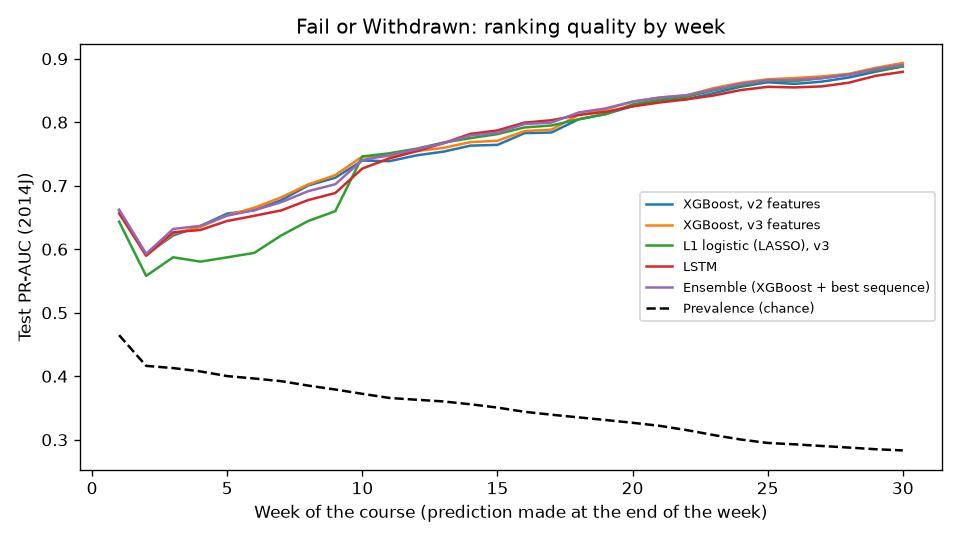
\includegraphics[width=\columnwidth]{figures/pr_auc_by_week.png}
\caption{Test PR-AUC by week for the Fail-or-Withdrawn outcome (OULAD 2014J); dashed line: base rate.}
\label{fig:week}
\end{figure}

\emph{Alert design.} With a threshold that maximises F1 on validation student-weeks, 98.2\% of adverse students
were alerted at least once, but so were 85.4\% of students who passed. Requiring two consecutive weeks reduced false
alarms by 0.099 [0.091, 0.107] but lost 18 points of recall; exponential smoothing kept recall (97.8\%) and cut alert
switches per student from 1.78 to 1.15. Monte Carlo dropout uncertainty tracked errors (Spearman 0.66): the most
certain 80\% of predictions had PR-AUC 0.805, the least certain 20\% only 0.520. Short-horizon withdrawal remained
hard (test PR-AUC 0.112 within 4 weeks, base rate 0.031); SMOTE never helped.

\subsection{Replications (Portugal)}
On UCI~697, dropout PR-AUC rose from 0.555 at enrolment to 0.797 after semester 1 (+0.241 [0.181, 0.298], Holm
$p=0.001$) and 0.836 after semester 2 (+0.040 [0.014, 0.067], $p=0.004$); LASSO and XGBoost did not differ at
semester 1 ($-0.012$ [$-0.032$, 0.009]). The strongest inputs were the semester-1 approval rate and the number of
failed units --- the analogue of backlogs in Indian colleges. Leaving out one of ten enrolment cohorts gave PR-AUC
0.77--0.87. Recall at semester 1 was 0.561 for women and 0.702 for men. Adding fee-status variables raised PR-AUC
at enrolment to 0.733; because their recording time is undocumented, this gain may come from information recorded
after students left, and we excluded them. On UCI~320 (L1 logistic, mean of $5\times5$ repeated cross-validation),
the first-period grade raised fail-prediction PR-AUC from 0.473 to 0.725 (Portuguese course; base rate 0.154).

\section{Discussion}
Across three datasets the strongest early signals are the first assessment results and submission behaviour ---
data that Indian colleges already hold as internal marks, assignments and backlogs. Simple, explainable models
were sufficient; the added complexity of sequence models was not repaid on these data. Two findings matter as much
as accuracy for deployment: fairness gaps vary by setting and must be audited for each institutional model, and
alert thresholds must be set per student over a term, or by mentor capacity, with uncertain cases routed to human
judgement. Limitations: all evidence is from UK and Portuguese benchmark data; OULAD contains no attendance; results
are associations, not causes; and no mentor study has yet been run. Real student data will be used only with
ethics approval, a data-sharing agreement and a lawful basis under India's Digital Personal Data Protection Act,
2023 \cite{dpdp2023}.

\section{Conclusion}
SEWS shows that an early-warning system can be built so that its evidence is trustworthy: leakage-checked
features, time-ordered and pre-registered evaluation, calibration and fairness audits, and a human decision on
every action. The next step is a retrospective study on one Indian college's anonymised past terms (technology
readiness level 5), followed by a one-semester pilot with mentors.

\begin{thebibliography}{99}
\bibitem{aishe} Ministry of Education, Government of India, ``All India Survey on Higher Education (AISHE)
2021-22,'' released Jan. 25, 2024.
\bibitem{arnold2012} K. E. Arnold and M. D. Pistilli, ``Course Signals at Purdue: Using learning analytics to
increase student success,'' in \emph{Proc. LAK '12}, 2012, pp. 267--270.
\bibitem{jayaprakash2014} S. M. Jayaprakash, E. W. Moody, E. J. M. Laur\'{\i}a, J. R. Regan, and J. D. Baron, ``Early
alert of academically at-risk students: An open source analytics initiative,'' \emph{J. Learning Analytics},
vol. 1, no. 1, pp. 6--47, 2014.
\bibitem{kuzilek2017} J. Kuzilek, M. Hlosta, and Z. Zdrahal, ``Open University Learning Analytics dataset,''
\emph{Scientific Data}, vol. 4, art. 170171, 2017.
\bibitem{hlosta2017} M. Hlosta, Z. Zdrahal, and J. Zendulka, ``Ouroboros: Early identification of at-risk students
without models based on legacy data,'' in \emph{Proc. LAK '17}, 2017, pp. 6--15.
\bibitem{herodotou2019} C. Herodotou, M. Hlosta, A. Boroowa, B. Rienties, Z. Zdrahal, and C. Mangafa,
``Empowering online teachers through predictive learning analytics,'' \emph{British J. Educational Technology},
vol. 50, no. 6, pp. 3064--3079, 2019.
\bibitem{gardner2018} J. Gardner and C. Brooks, ``Student success prediction in MOOCs,'' \emph{User Modeling and
User-Adapted Interaction}, vol. 28, pp. 127--203, 2018.
\bibitem{namoun2021} A. Namoun and A. Alshanqiti, ``Predicting student performance using data mining and learning
analytics techniques: A systematic literature review,'' \emph{Applied Sciences}, vol. 11, no. 1, art. 237, 2021.
\bibitem{glandorf2024} D. Glandorf, H. R. Lee, G. A. Orona, M. Pumptow, R. Yu, and C. Fischer, ``Temporal and
between-group variability in college dropout prediction,'' in \emph{Proc. LAK '24}, 2024.
\bibitem{le2026} N. L. Le, M.-H. Abel, and B. Laforge, ``When can we trust early warnings? Leakage-excluded early
outcome prediction from LMS interaction logs,'' arXiv:2605.25794, 2026 (preprint).
\bibitem{kaufman2012} S. Kaufman, S. Rosset, C. Perlich, and O. Stitelman, ``Leakage in data mining: Formulation,
detection, and avoidance,'' \emph{ACM Trans. Knowledge Discovery from Data}, vol. 6, no. 4, 2012.
\bibitem{gardner2019} J. Gardner, C. Brooks, and R. Baker, ``Evaluating the fairness of predictive student models
through slicing analysis,'' in \emph{Proc. LAK '19}, 2019, pp. 225--234.
\bibitem{baker2022} R. S. Baker and A. Hawn, ``Algorithmic bias in education,'' \emph{Int. J. Artificial
Intelligence in Education}, vol. 32, no. 4, pp. 1052--1092, 2022.
\bibitem{yu2021} R. Yu, H. Lee, and R. F. Kizilcec, ``Should college dropout prediction models include protected
attributes?'' in \emph{Proc. ACM L@S '21}, 2021.
\bibitem{khosravi2022} H. Khosravi \emph{et al.}, ``Explainable artificial intelligence in education,''
\emph{Computers and Education: Artificial Intelligence}, vol. 3, art. 100074, 2022.
\bibitem{lundberg2017} S. M. Lundberg and S.-I. Lee, ``A unified approach to interpreting model predictions,'' in
\emph{Advances in Neural Information Processing Systems 30}, 2017, pp. 4768--4777.
\bibitem{chen2016} T. Chen and C. Guestrin, ``XGBoost: A scalable tree boosting system,'' in \emph{Proc. KDD '16},
2016, pp. 785--794.
\bibitem{niculescu2005} A. Niculescu-Mizil and R. Caruana, ``Predicting good probabilities with supervised
learning,'' in \emph{Proc. ICML '05}, 2005, pp. 625--632.
\bibitem{realinho2021} V. Realinho, M. Vieira Martins, J. Machado, and L. Baptista, ``Predict students' dropout and
academic success,'' UCI Machine Learning Repository, 2021, doi: 10.24432/C5MC89.
\bibitem{cortez2008} P. Cortez and A. M. G. Silva, ``Using data mining to predict secondary school student
performance,'' in \emph{Proc. 5th Future Business Technology Conf.}, 2008; dataset: UCI Machine Learning
Repository, doi: 10.24432/C5TG7T.
\bibitem{page1954} E. S. Page, ``Continuous inspection schemes,'' \emph{Biometrika}, vol. 41, no. 1/2,
pp. 100--115, 1954.
\bibitem{tibshirani1996} R. Tibshirani, ``Regression shrinkage and selection via the lasso,'' \emph{J. Royal
Statistical Society B}, vol. 58, no. 1, pp. 267--288, 1996.
\bibitem{cho2014} K. Cho \emph{et al.}, ``Learning phrase representations using RNN encoder--decoder for
statistical machine translation,'' in \emph{Proc. EMNLP}, 2014, pp. 1724--1734.
\bibitem{hochreiter1997} S. Hochreiter and J. Schmidhuber, ``Long short-term memory,'' \emph{Neural Computation},
vol. 9, no. 8, pp. 1735--1780, 1997.
\bibitem{bai2018} S. Bai, J. Z. Kolter, and V. Koltun, ``An empirical evaluation of generic convolutional and
recurrent networks for sequence modeling,'' arXiv:1803.01271, 2018.
\bibitem{chawla2002} N. V. Chawla, K. W. Bowyer, L. O. Hall, and W. P. Kegelmeyer, ``SMOTE: Synthetic minority
over-sampling technique,'' \emph{J. Artificial Intelligence Research}, vol. 16, pp. 321--357, 2002.
\bibitem{singer1993} J. D. Singer and J. B. Willett, ``It's about time: Using discrete-time survival analysis to
study duration and the timing of events,'' \emph{J. Educational Statistics}, vol. 18, no. 2, pp. 155--195, 1993.
\bibitem{harrell1982} F. E. Harrell, R. M. Califf, D. B. Pryor, K. L. Lee, and R. A. Rosati, ``Evaluating the yield
of medical tests,'' \emph{JAMA}, vol. 247, no. 18, pp. 2543--2546, 1982.
\bibitem{gal2016} Y. Gal and Z. Ghahramani, ``Dropout as a Bayesian approximation: Representing model uncertainty
in deep learning,'' in \emph{Proc. ICML}, 2016, pp. 1050--1059.
\bibitem{delong1988} E. R. DeLong, D. M. DeLong, and D. L. Clarke-Pearson, ``Comparing the areas under two or more
correlated receiver operating characteristic curves: A nonparametric approach,'' \emph{Biometrics}, vol. 44,
no. 3, pp. 837--845, 1988.
\bibitem{holm1979} S. Holm, ``A simple sequentially rejective multiple test procedure,'' \emph{Scandinavian J.
Statistics}, vol. 6, pp. 65--70, 1979.
\bibitem{dpdp2023} \emph{The Digital Personal Data Protection Act, 2023}, Government of India.
\end{thebibliography}

\end{document}
